%%%%%%%%%%%%%%%%%%%%%%%%%%%%%%%%%%%%%%%%%%%%%%%%%%%%%%%%%%%%%%%%%%%%%%
% How to use writeLaTeX: 
%
% You edit the source code here on the left, and the preview on the
% right shows you the result within a few seconds.
%
% Bookmark this page and share the URL with your co-authors. They can
% edit at the same time!
%
% You can upload figures, bibliographies, custom classes and
% styles using the files menu.
%
%%%%%%%%%%%%%%%%%%%%%%%%%%%%%%%%%%%%%%%%%%%%%%%%%%%%%%%%%%%%%%%%%%%%%%

\documentclass[12pt]{article}

\usepackage{sbc-template}

\usepackage[alf]{abntex2cite}
\bibliographystyle{abntex2-alf}

\usepackage[caption=false]{subfig}

\usepackage[section]{placeins}

\usepackage{quoting}

\usepackage{graphicx}

\usepackage[export]{adjustbox}

\usepackage[brazil]{babel} 

\usepackage[utf8]{inputenc}  
     
\sloppy

\title{Análise de Usabilidade do Portal Acadêmico UCSal}

\author{Renan Torrentes C. de Paula\inst{1}, Ronilson M. Lobo\inst{2} }


\address{Análise e Desenvolvimento de Sistemas -- Universidade Católica do Salvador
  (UCSal)\\
 Av. Prof. Pinto de Aguiar, 2589 -- Pituaçu -- 41.740-090 -- Salvador -- BA --  Brazil
 \nextinstitute
 Dep. de Comunicação e Computação -- Universidade Católica do Salvador (UCSal)\\Salvador -- BA -- Brazil
 \email{renan.paula@ucsal.edu.br, ronilson.lobo@pro.ucsal.br}
}

\begin{document} 

\maketitle

\begin{abstract}
  This work presents an analysis of the usability of the Catholic University of Salvador (UCSal) Academic Portal and a prototype. Thus, we performed bibliographic research and we applied a questionnaire to the students of the institution. To achieve our goal, we took a brief tour of the internet history from its evolution to the current studies of Human-Computer Interaction (HCI). According to this theory, we focus on the concept of usability and we use it for the analysis of the portal added the interviewed students’ answers. As a result, we concluded the Portal needs to be focused on the user and the usability criteria must be applied in order that they can work efficiently. To exemplify how this result should be applied to the Academic Portal, we present a Prototype in order to materialize the research result's and theory presented here. This work opens the doors to studies in several theories within Information Technology.
\end{abstract}
     
\begin{resumo} 
  Este artigo objetiva apresentar uma análise da usabilidade do Portal Acadêmico da Universidade Católica do Salvador (UCSal) e, também, um protótipo. Para isso, realizamos pesquisas bibliográficas e aplicamos um questionário para os alunos da instituição. A fim de alcançar os objetivos, fizemos um breve percurso da história da Internet da sua evolução até os estudos atuais da Interação Homem-Computador (IHC). Nessa teoria, focamos no conceito de usabilidade e o utilizamos para a análise do portal somado com as respostas dos alunos entrevistados. Como resultado da pesquisa, concluímos que o Portal precisa ser focado no usuário e os critérios de usabilidade devem ser aplicados para que possam funcionar de maneira eficiente. Para exemplificar como esse resultado deveria ser aplicado no Portal, apresentamos um Protótipo com o objetivo de materializar o resultado da pesquisa e a teoria aqui apresentada. Este trabalho abre caminhos para estudos em diversas teorias dento da Tecnologia da Informação.
\end{resumo}


\section{Introdução}
O objeto de estudo deste trabalho é o Portal Acadêmico da Universidade Católica do Salvador (UCSal), ferramenta que é utilizada por todos os alunos da instituição (Graduação e Pós-graduação). 

Esta pesquisa objetiva analisar a usabilidade do Portal da UCSal. Para alcançar este objetivo, foram realizadas: pesquisas bibliográficas sobre o referencial teórico; pesquisa entre os alunos da universidade a fim de constatar a impressão que esses têm do Portal; aplicação de testes de usabilidade em cima dos resultados da pesquisa e sugestões de melhorias (protótipo) a partir da avaliação de resultados dos itens citados anteriormente.

O trabalho proposto está no nível descritivo e pode ser classificado como uma pesquisa bibliográfica, pois a nossa fonte de consulta foram materiais já elaborados (Livros, artigos científicos etc.). Este também pode ser classificado como um levantamento pois, como já mencionado anteriormente, será aplicado um questionário para os alunos da instituição avaliarem o Portal.

A estrutura do artigo será composta na seguinte ordem:  No capítulo 2, apresentação do referencial teórico, em que abordaremos o que autores como Barbosa e Silva (2010) tratam sobre o tema Interação Homem-Computador e Usabilidade; no capítulo 3, apresentaremos a metodologia utilizada para analisar o portal; no subtópico 3.1 apresentaremos o objeto de estudo desse trabalho.

No capítulo 4, analisaremos o Portal do aluno UCSal e o relacionaremos com a teoria apresentada no capítulo 2 e com o resultado da pesquisa feita com os alunos da instituição, evidenciando os resultados negativos e positivos de nossa análise.

Em seguida, no capítulo 5, mostraremos as sugestões de melhorias para o nosso objeto de estudo tendo como base o referencial teórico e, sobretudo, a opinião dos alunos, dentro do que for previsto pela teoria e apresentaremos um protótipo desenvolvido utilizando a ferramenta Adobe XD para demonstrar as melhorias propostas em um exemplo visual.

Por fim,  apresentaremos as Considerações finais onde evidenciaremos o resultado desta pesquisa e ressaltamos que a sua contribuição pode ser uma das bases para outros trabalhos na mesma linha. 
\section{Referencial Teórico} \label{refTeorico}
Para alcançarmos o objetivo deste trabalho, escolhemos como ponto de partida o surgimento da Internet. 
Essa, segundo \citeonline{silva_internet} foi criada no ano de 1969 nos Estados Unidos (EUA), conhecida como Arpanet, ela tinha como principal função, interligar institutos de pesquisa. Naquele momento, o mundo passava pela Guerra Fria, e a Arpanet surgiu como uma garantia de que, mesmo em caso de bombardeios, a comunicação entre militares e cientistas iria persistir. Dezoito anos após o seu surgimento, o uso comercial da internet foi liberado. Até esse momento, apenas a comunidade acadêmica e cientifica tinham acesso à rede.

De acordo com \citeonline{agencia_ex2_web_2013}, o primeiro Browser (Navegador) surgiu no início da década de 90 e tinha como objetivo servir como uma ferramenta que centralizava as tarefas necessárias para se obter as informações disponíveis na internet. O WWW (World Wide Web) atraiu usuários de todo mundo por conta da simplicidade pela qual ela disponibilizava o conteúdo da internet e a partir daí a difusão da rede foi enorme e com um crescimento exponencial de usuários.

A mesma Agência afirma que, desde a sua criação, a internet está em constante evolução e a sua trajetória até o momento foi categorizada em 3 gerações. A primeira geração foi chamada de WEB 1.0, teve início no ano de 1990 e durou até 2003, foi caracterizada por seu conteúdo estático e por não oferecer nenhuma forma de interatividade com os usuários, ou seja, era uma via de comunicação de mão única. 

No ano de 2003, segundo o \citeonline{oreilly_what_2005},  Dale Dougherty utilizou pela primeira vez o termo WEB 2.0. com o foco direcionado para os usuários, as redes sociais ganham força e uma variedade de serviços e facilidades são oferecidas.  O que antes era estático, passa agora ser dinâmico, promovendo a colaboração entre os usuários a geração de conteúdo na web cresce exponencialmente e as informações passam a estar disponíveis o tempo todo e para todos. 

O jornalista John Markoff, em um artigo do New York Times citou o termo WEB 3.0 pela primeira vez, de acordo com \citeonline{davila_folha_2007}. Essa é a internet mais atual e consiste em uma internet além da interatividade, conhecida como a “Web Inteligente” ou “Web Semântica”, termo cunhado por "[...] Tim Berners-Lee, James Hendler e Ora Lassila a partir de uma preocupação em relação ao grande crescimento desenfreado da internet tomando proporções inimagináveis."  \cite{becker_o_2019}.

A internet agora passa a focar no uso das máquinas e algoritmos para oferecer conteúdo personalizado aos usuários. Dessa forma, é possível oferecer ajuda em tempo real aos usuários, através da Inteligência Artificial; o uso dos dispositivos móveis e IOT (Internet of Things) proporcionou uma maior interação com a rede, deixando os usuários conectados 24 horas  durante os 7 dias da semana. Com isso, o uso dos Smartphones, Smart-Tvs,\textit{ Smart-Houses}, carros, videogames e \textit{wearables} geram uma massa absurda de dados que são consumidos pelos algoritmos, que passam a entender cada vez mais as nossas necessidades enquanto pessoa e consumidor e fornecem conteúdos de maior relevância para os usuários. 

A Tecnologia da Informação (TI), conforme afirmam \citeonline{barbosa}, vem se desenvolvendo em ritmo acelerado e faz cada vez mais parte de nossas vidas pessoais e profissionais. A disseminação dessas tecnologias alcançou um nível em que é muito difícil encontrar pessoas que ainda não tiveram, mesmo que indiretamente, um contato com elas, independente de classe social, escolaridade ou fator cultural.
Diante desse cenário,  \citeonline[p. ~9]{morais} dizem que:
\begin{quoting}[rightmargin=0cm,leftmargin=4cm]
{\footnotesize 
Essa utilização maçante e repentina tem causado várias discussões entre os desenvolvedores de aplicativos, sobre como criar ferramentas que facilitem a utilização e a satisfação dos seus usuários, atraindo cada vez mais “clientes” para sua aplicação. Em razão dessa necessidade de mercado, os estudos na área de Interação Homem-Computador (IHC) foram intensificando. Nesse contexto, a partir das funcionalidades das aplicações, o foco geralmente está direcionado à satisfação do usuário. Essa satisfação pode ser definida pela qualidade de uma interação entre o ser humano e o computador.}	
\end{quoting}

Essa demanda pela qualidade na interação do homem com os sistemas computacionais gerou a necessidade de fornecer técnicas e diretrizes de avaliação de IHC, que acabaram por se tornar guias para a condução da criação de interfaces. Ao seguir esses guias, é possível detectar e solucionar possíveis problemas de interação. Segundo \citeonline{barbosa}, usar um sistema interativo significa interagir com a sua interface a fim de alcançar objetivos em um determinado contexto de uso.

A partir do exposto, podemos constatar que a internet saiu de uma fase estática para uma fase de inclusão e interação e continua em constante desenvolvimento. Para que a rede mundial de computadores e os seus frutos continuem evoluindo é fundamental adaptar as plataformas existentes ao conceito da Arquitetura da Informação. 

\subsection{Arquitetura da Informação}
Essa é definida pelo The Information Architecture Institute (Instituto de Arquitetura da Informação) como “\textit{is the practice of deciding how to arrange the parts of something to be understandable}.”. Em uma tradução nossa “é a prática de decidir como organizar as partes de algo para ser compreensível.”.

Para entender a importância desse conceito para a internet, veja a analogia abaixo:
\begin{quoting}[rightmargin=0cm,leftmargin=4cm]
{\footnotesize 
Se você for a um supermercado pela primeira vez e quiser saber onde ficam os chocolates, provavelmente vai procurar por uma placa que indica a seção de doces e sobremesas. Da mesma forma, se quiser consultar os ingredientes de um produto, é de se esperar que consiga encontrar essa informação com facilidade na embalagem.
O mesmo vale para o mundo digital [...] — basta adaptar o conceito para softwares, aplicativos, sites, blogs etc.
É fundamental que eles contenham as informações em uma estrutura facilmente compreensível, que siga uma lógica simples e que leve em consideração as possibilidades de interação. \cite{xavier_arquitetura}}
\end{quoting}

O autor mencionado acima, destaca que a Arquitetura da Informação atua em 03 campos: do conteúdo; dos usuários e do contexto. Neste trabalho, sem dispensar a importância de análise dos outros dois, focaremos no campo do usuário. Por isso, no tópico seguinte, abordaremos alguns conceitos da Interação Humano-Computador.

\subsection{Interação Humano-Computador}
As inúmeras tecnologias que temos acesso são analisadas com diferentes perspectivas pelos membros da sociedade. Exemplo: um aplicativo de uma clínica será avaliado de uma maneira pelo setor administrativo, por outra maneira pelos médicos, pelos pacientes etc.
Essa mesma análise diverge mesmo entre aqueles que trabalham diretamente com o desenvolvimento da tecnologia.
\begin{quoting}[rightmargin=0cm,leftmargin=4cm]
{\footnotesize 
Grande parte da Computação e, em particular, a subárea de Engenharia de Software, está interessada na construção de sistemas interativos mais eficientes, robustos, livres de erros, e de fácil manutenção. Por outro lado, a área de Interação Humano-Computador (IHC) está interessada na qualidade de uso desses sistemas e no seu impacto na vida dos seus usuários. Apesar de fortemente relacionados, a construção e o uso de um artefato ocorrem em contextos distintos e seguem lógicas diferentes, envolvendo pessoas diversas. \cite[p. ~29-30]{barbosa}}
\end{quoting}

Neste trabalho, nos interessa o foco da IHC no que tange ao impacto dos sistemas para os usuários, pois acreditamos que é necessário analisar como a tecnologia está sendo usada e entendida pelo público. Afinal, "Se seguirmos uma abordagem de 'dentro para fora', corremos um grande risco de concebermos um sistema interativo inapropriado para o mundo que o cerca, pois a nossa compreensão do mundo pode ser equivocada."  \cite[p. ~30]{barbosa}.

Nos estudos da IHC é possível encontrar a definição de 03 situações: Interação, Interface; e \textit{Affordance}. 

Interação é descrita “como tudo o que acontece quando uma pessoa e um sistema computacional se unem para realizar tarefas, visando a um objetivo.” \apud[p.~43]{hix}{barbosa}.

Já Interface “compreende toda a porção do sistema com a qual o usuário mantém contato físico (motor ou perceptivo) ou conceitual durante a interação." \apud[p.~48]{moran}{barbosa}.

O nosso destaque aqui vai para o termo \textit{Affordance}. Definido como “o conjunto de características do hardware e do software perceptíveis pelo usuário aponta para um conjunto de operações que podem ser realizadas com o sistema interativo, bem como para as formas de realizá-las manipulando os elementos da interface.”. \cite[p. ~49]{barbosa}

A importância desse conceito está no fato de que a partir dele é possível que o usuário perceba tudo que é possível fazer no sistema. Para que o usuário identifique tal característica é de extrema importância que tenha sido implantado, no site ou no aplicativo, os critérios de qualidade em IHC (termo similiar à qualidade de uso).

\citeonline{barbosa} apresentam 04 critérios de qualidade de uso. São eles: comunicabilidade, acessibilidade, experiência do usuário e usabilidade. Como já mencionamos anteriormente, neste trabalho, utilizaremos o conceito de usabilidade para análise do portal do aluno sem deixar de considerar a experiência de usuário.

\subsubsection{Usabilidade}
Com as inúmeras possibilidades de navegação que o usuário tem à sua disposição, caso ele possa escolher, ele sempre optará por sites e aplicativos que sejam mais simples, intuitivos e rápidos. Por esses motivos, atualmente, há inúmeros estudos focados no usuário. 
\begin{quoting}[rightmargin=0cm,leftmargin=4cm]
{\footnotesize 
A usabilidade (ou falta dela) é um componente muito importante de um website, e que pode significar o sucesso ou insucesso do mesmo junto dos seus utilizadores. Uma má experiência de utilização pode fazer com que os utilizadores desistam de usar o website e comecem a usar o site da concorrência.  \cite{noauthor_introducao_usabilidade}}
\end{quoting}
Atualmente, não é suficiente que o site ou \textit{app} ofereça o que ele promete. Por exemplo: um site que vende roupas. Podem ser disponibilizadas fotografias das peças, preços, diversos tamanhos etc. Tudo que o cliente precisa para fazer a compra. Mas se o \textit{layout} for confuso, as frases não forem objetivas, os ícones não corresponderem ao que realmente representam, haverá uma dificuldade de navegação e isso pode até mesmo fazer com que o cliente desista da compra.  

Dentro de usabilidade não podemos descartar a experiência do usuário, afinal “ [...] a usabilidade passou a englobar também as emoções e os sentimentos dos usuários.” \cite[p. ~51]{barbosa}.

Para saber sobre essa experiência, sentimos a necessidade aplicar um questionário aos alunos da UCSal, porque só a partir da percepção deles será possível alcançarmos os objetivos deste trabalho.

A existência da norma ISO/IEC 9126 descreve que é preciso considerar em um sistema a sua eficácia e eficiência.  A primeira se trata do usuário alcançar os seus objetivos conforme ele espera, a segunda se relaciona com a disponibilização dos recursos para que os usuários possam interagir com o site/\textit{app} e, além disso, consigam concretizar a sua ação.

Além dos critérios mencionados na norma acima, ela ainda fala sobre satisfação. Algo que  pode ser relacionado com a experiência do usuário, mas que sabemos que nem sempre será positiva.

Para análise do \textit{corpus}, utilizaremos os fatores de usabilidade mencionados pelo \citeonline{nielsen}. A saber: Learnability (Facilidade de aprendizado); Efficiency (Eficiência); Memorability (Facilidade de recordação); Safety (Segurança no uso) e Satisfaction (Satisfação do usuário). Optamos por descrever esses fatores à medida em que eles apareçam na análise, assim como outros que possam se relacionar com usabilidade e com o objeto de estudo.
\section{Metodologia\label{sec:metodologia}}
A pesquisa proposta pode ser definida como descritiva, em que “tem por objetivo descrever as características de uma população, de um fenômeno ou de uma experiência. Esse tipo de pesquisa estabelece relação entre as variáveis no objeto de estudo analisado. Variáveis relacionadas à classificação, medida e/ou quantidade que podem se alterar mediante o processo realizado.” \cite{duarte}.

Quanto a sua classificação, se trata de uma pesquisa bibliográfica, pois a nossa fonte de consulta foram materiais já elaborados (Livros, artigos científicos etc.). 

Por considerarmos a experiência do usuário fundamental para a analisarmos a usabilidade do Portal do Aluno, realizamos uma pesquisa de opinião com os alunos da UCSal, aplicada em forma de questionário na plataforma do Google Forms, onde obtivemos um total de 63 participantes. 

Com base nas informações encontradas no Ranking Universitário 2019, \citeonline{folha_de_sao_paulo_universidade_2019}, a UCSal possui 8.686 alunos. Número utilizado para calcular a margem de erro e o grau de confiança da pesquisa. Para conhecermos esses resultados, utilizamos a calculadora de plano amostral do site \citeauthoronline{noauthor_calculadora}. Nele, obtivemos uma margem de erro de 12\% e um grau de confiança de 95\% em nossa pesquisa, e com isso o trabalho também pode ser classificado além de bibliográfico como uma pesquisa de levantamento. 

No questionário aplicado através do Google Forms, foram feitas perguntas para conhecer o perfil do aluno entrevistado, porém para este trabalho os questionamentos que possuem impacto significativo foram: Como você acessa o portal do aluno da UCSAL?/ Por qual dispositivo você acessa o Portal?/ Qual a sua prioridade ao acessar o portal?/ Os textos exibidos estão bem formatados e alinhados./ A linguagem é clara e objetiva./ É possível se situar facilmente no portal durante a navegação./ Os ícones estão coerentes com os seus respectivos textos (Tela inicial)./ Os ícones estão coerentes com os seus respectivos textos (Menu lateral)./ O acesso ao portal pelo celular é de fácil navegação./ O portal é responsivo (Se adapta ao tamanho da tela do celular)./ O Design do portal é moderno./ A navegação no portal é intuitiva e simples.

A formulação do questionário  seguiu as diretrizes do modelo de Avaliação de IHC através de observação. Esse método de avaliação permite ao avaliador coletar dados sobre situações em que os participantes utilizam um sistema tecnológico. A análise desses dados ajuda a identificar problemas reais que os usuários enfrentam. Dentro deste modelo, utilizamos o conceito de Teste de usabilidade para formular as perguntas do questionário.

\subsection{Teste de Usabilidade} 
O Teste de Usabilidade “[...] visa a avaliar a usabilidade de um sistema interativo a partir de experiências de uso dos seus usuários-alvo.” \apud[p.~365]{rubin}{barbosa}. Essa avaliação tem como objetivo determinar quais os critérios de usabilidade devem ser analisados. 

Sendo assim, o resultado obtido através dos questionários servirá como base para a análise da usabilidade do nosso objeto de estudo.

\subsection{O Objeto de Estudo}
Para conhecimento do \textit{corpus }apresentamos abaixo duas imagens, o menu de opções inicial e a tela principal do Portal.

\begin{figure}[!htb]
\centering
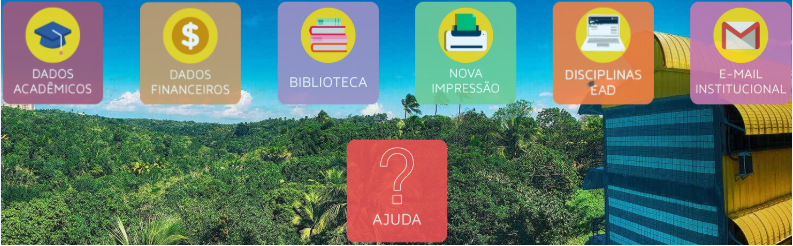
\includegraphics[scale=0.35,frame]{img1.png}
\caption{Tela Inicial}
\label{fig:imgTelaInicial}
\end{figure}

\begin{figure}[!htb]
\centering
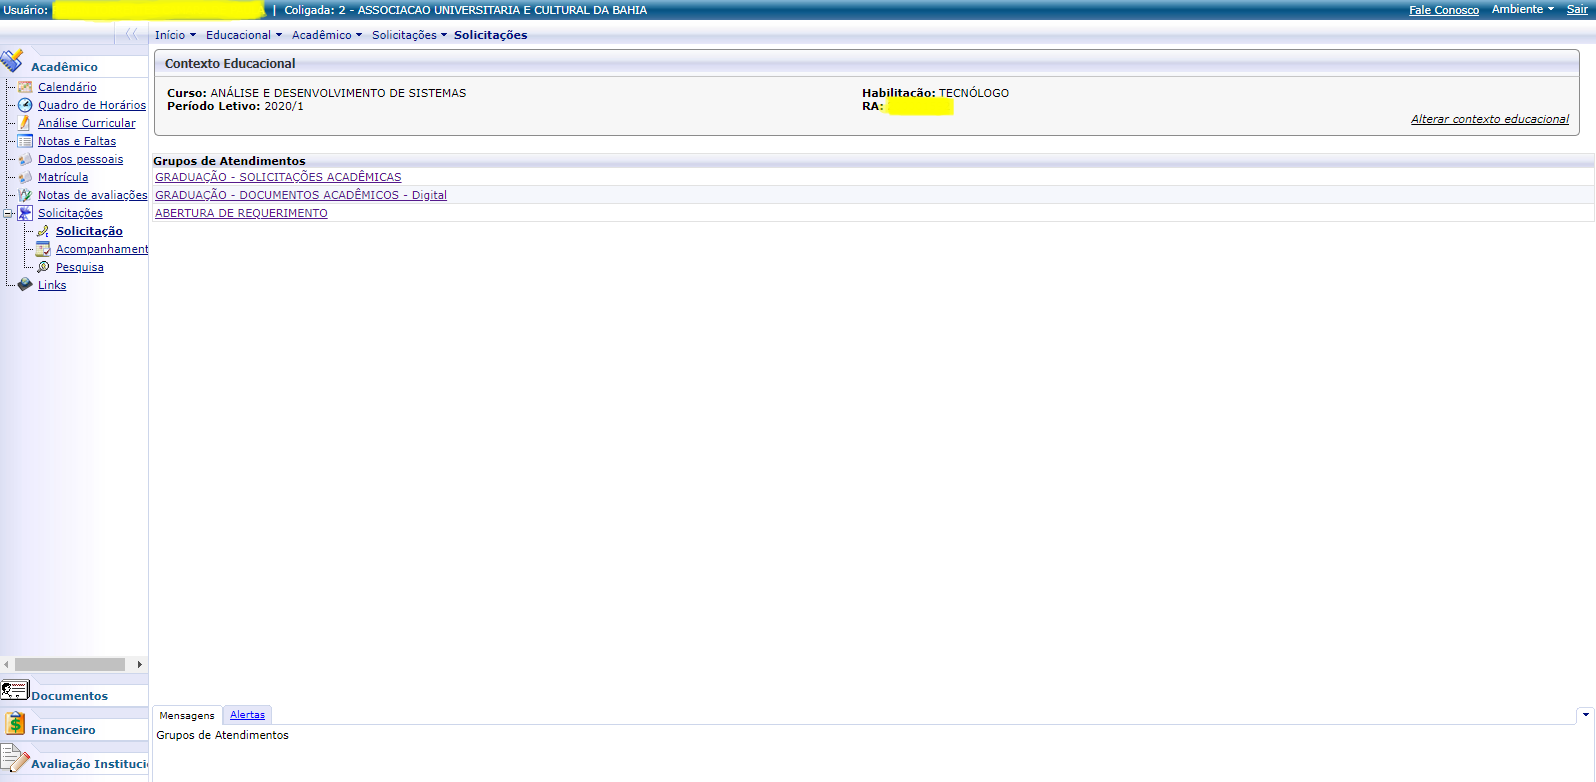
\includegraphics[scale=0.25,frame]{img2.png}
\caption{O Portal}
\label{fig:imgOPortal}
\end{figure}
\FloatBarrier
\section{Análise do Portal UCSal\label{sec:analiseportal}}
O Portal da UCSal é a principal ferramenta tecnológica de interação entre os alunos da instituição com a Universidade Católica do Salvador. Nele é possível acessar os dados acadêmicos, financeiros, biblioteca, disciplinas EAD (Educação À Distância), realizar impressão de arquivos e responder a pesquisas institucionais da Universidade. 

Para iniciarmos a análise, definimos 3 pontos de partida com base nas primeiras questões da pesquisa com os alunos: Como o aluno acessa o Portal? Por onde acessa o Portal e quais as prioridades de utilização no acesso ao Portal.

\begin{figure}[!htb]
\centering
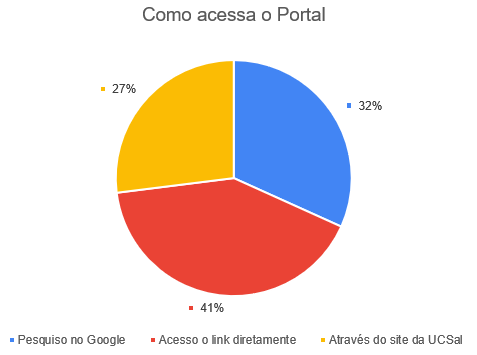
\includegraphics[scale=0.4,frame]{img3.png}
\caption{Como o aluno acessa o Portal}
\label{fig:grafico1}
\end{figure}

Como é possível observar na Figura 3, 41\% dos alunos acessam o portal através do seu endereço direto, ou seja, digitam o endereço do portal na barra do navegador. Isso evidencia que o acesso a ferramenta é feito constantemente, podemos até inferir que este endereço pode já estar salvo em seus navegadores, facilitando ainda mais o acesso ao site.

Aproveitamos essa pergunta para expor algo observado no site oficial da UCSal. Embora ele não seja o nosso objeto de estudo, o problema identificado pode ser a causa de sites de buscas serem a 2ª forma mais utilizada de acesso ao Portal.  Confira a tela principal do site na Figura 4: 

\begin{figure}[!htb]
\centering
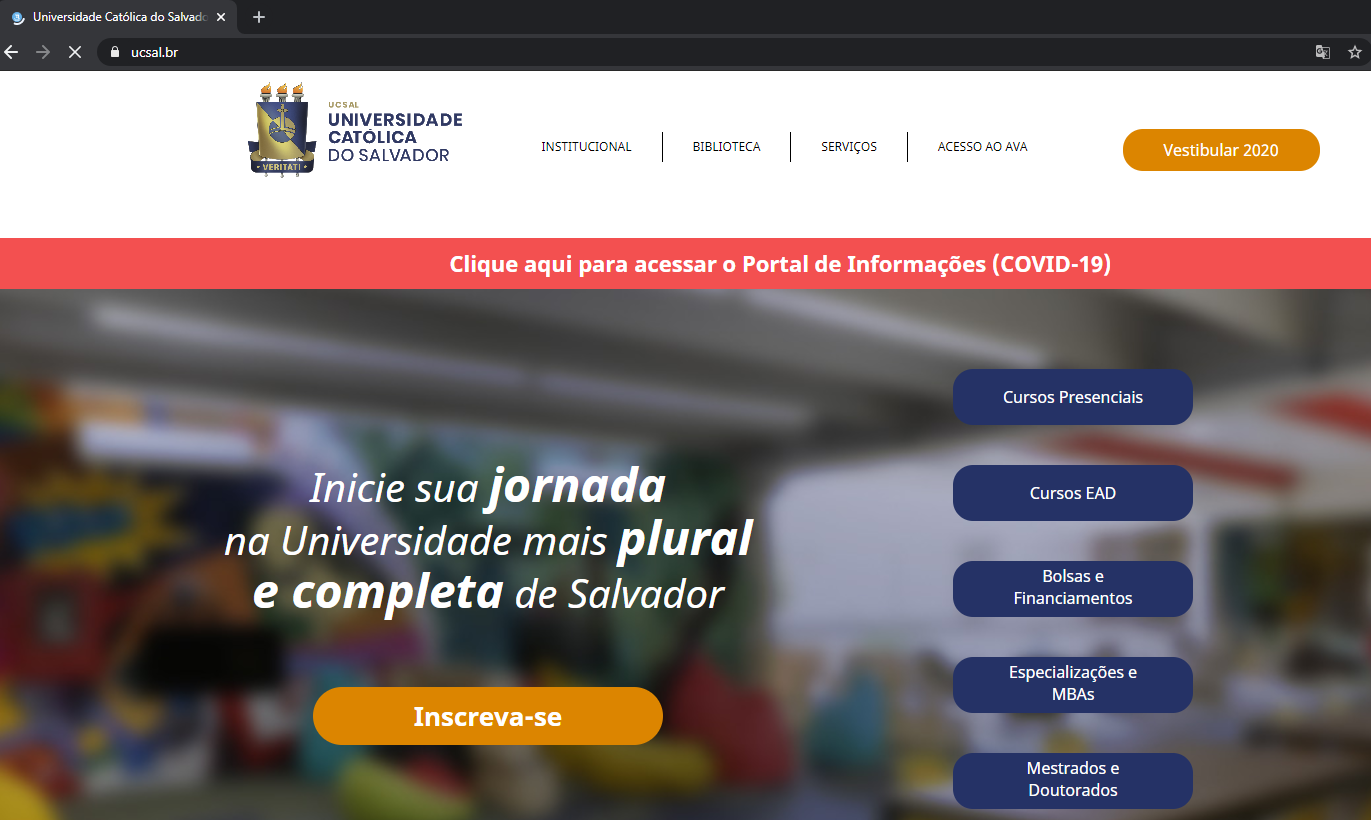
\includegraphics[scale=0.25,frame]{img4.png}
\caption{Site da UCSal}
\label{fig:siteucsal}
\end{figure}

Observe que não há explicitamente, na tela principal, a opção de acesso ao Portal do Aluno. Esse acesso não disponibilizado de maneira simples e objetiva no site da Universidade pode ser caracterizado como um problema no critério de usabilidade em IHC. Logo, se o usuário não tiver afinidade com o site da UCSal, a maneira mais fácil de acessar o Portal será pelo site de busca. 

\begin{figure}
	\centering    
	\begin{minipage}{.4\columnwidth}
		\centering    
		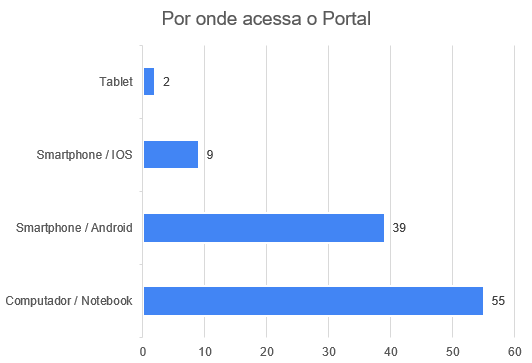
\includegraphics[width=\textwidth,frame]{img5.png}
		\caption{Formas mais utilizadas para acessar o Portal}
		\label{fig:grafico2}
	\end{minipage}
	\begin{minipage}{.4\columnwidth}
		\centering
		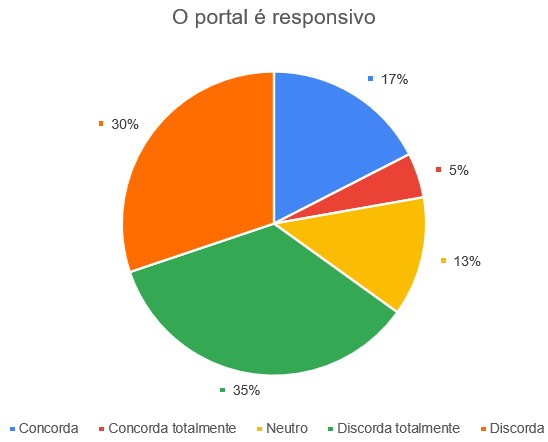
\includegraphics[width=\textwidth,frame]{img6.png}
		\caption{Responsividade do Portal}
		\label{fig:grafico3}
	\end{minipage}
\end{figure}

Nosso segundo ponto foi identificar por qual dispositivo os alunos acessam o Portal. Como evidenciado na Figura 5, a maioria dos acessos é realizado através de um Computador ou Notebook. Para essa pergunta, os alunos entrevistados poderiam marcar mais de uma opção. Os acessos através de um smartphone Android também aparecem de forma significativa em nossa pesquisa. Isso acontece devido ao avanço da tecnologia que já mencionamos anteriormente. Este inclusive foi um dos pontos que nos levaram a realizar essa análise de interface, pois como confirmado na Figura 6, o Portal do Aluno não se adapta ao tamanho das telas dos celulares ou tablets. Ou seja, o Portal não é responsivo.

Responsividade é a capacidade que um site tem de se adaptar a diferentes tamanhos de telas através da reorganização do conteúdo, imagens e simplificação do menu de acordo com \citeonline{noauthor_webresponsiva}. Essa característica é muito importante na atualidade, pois a utilização dos smartphones para navegar na internet já é uma tendência no mundo todo. 

A falta de responsividade no Portal da UCSal se torna uma fator que dificulta o seu acesso através dos dispositivos mais utilizados pelos alunos. 

Como citamos anteriormente, quando o usuário tem a opção de navegar em sites adaptados essa será a sua principal opção. Porém, destacamos que, no caso dos alunos da UCSal, eles não possuem outra alternativa a não ser navegar por uma ferramenta que não se adapta ao seu dispositivo.  A responsividade, nesse cenário, é algo que influencia diretamente em um dos critérios de usabilidade que analisaremos em seguida: Satisfação do usuário.

Segundo \citeonline{nielsen}, Satisfação do usuário pode ser definida sobre o quão agradável é de se utilizar um sistema. No cenário acima, a experiência do usuário é afetada durante a utilização do sistema através de um smartphone, pois para conseguir ler e navegar no Portal o usuário precisa redimensionar a tela manualmente, o que torna a utilização do sistema não agradável. Isso pode ser confirmado na Figura 7,  em que mais de 65\% dos entrevistados discordam que o Portal tenha uma navegação fácil pelo celular:

\begin{figure}[!htb]
\centering
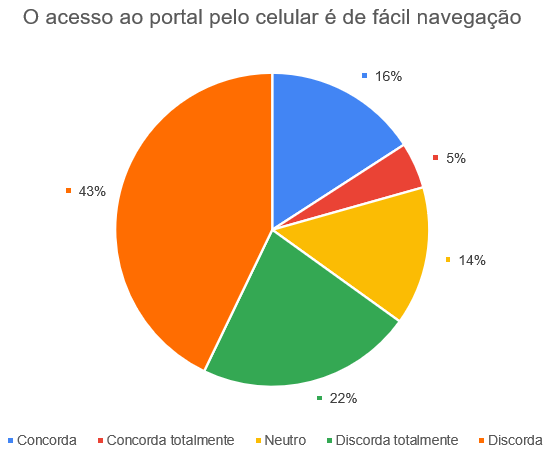
\includegraphics[scale=0.4,frame]{img7.png}
\caption{Facilidade de navegação pelo celular}
\label{fig:grafico4}
\end{figure}
\FloatBarrier
Essa dificuldade de acesso pelo celular, além de não ter um design responsivo, se relaciona com a falta do design moderno avaliado por 62\% dos alunos como ultrapassado, como evidenciado na Figura 8.

Outro ponto analisado foi a prioridade de uso do sistema ao acessar o Portal do Aluno. Os resultados apontam que a maioria dos alunos que acessam o Portal tem como maior prioridade a utilização da ferramenta para fins acadêmicos. Em seguida, como prioridade média, o acesso aos dados financeiros e como prioridade baixa, o acesso a biblioteca institucional online, conforme demonstra a Figura 9.
\begin{figure}
	\centering    
	\begin{minipage}{.4\columnwidth}
		\centering    
		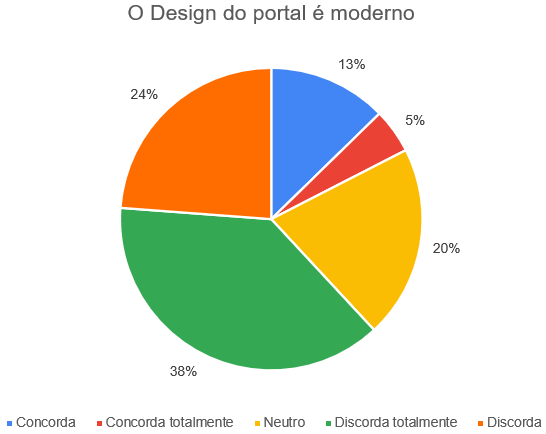
\includegraphics[width=\textwidth,frame]{img8.png}
		\caption{Design do Portal}
		\label{fig:grafico5}
	\end{minipage}
	\begin{minipage}{.45\columnwidth}
		\centering
		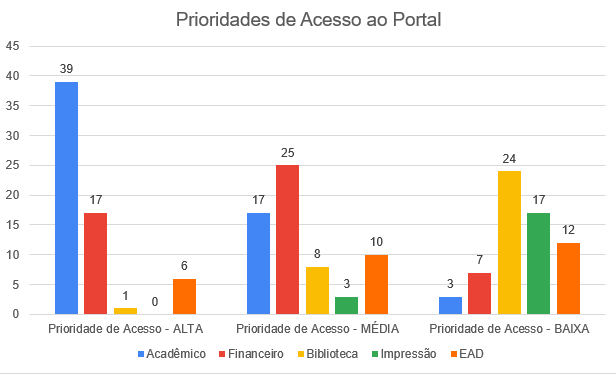
\includegraphics[width=\textwidth,frame]{img9.png}
		\caption{Prioridade de acesso}
		\label{fig:grafico6}
	\end{minipage}
\end{figure}

É importante destacarmos que as categorias: Biblioteca, Disciplinas EAD e Impressão não fazem parte do Portal do Aluno em si, essas ferramentas estão disponíveis em outros locais, servindo ao portal apenas a função de agregar os endereços e redirecionar os alunos a esses serviços.

Um dos critérios de Usabilidade identificados nessa análise é a Facilidade de recordação. Ele pode ser definido como a facilidade a qual o sistema tem de ser memorizado/lembrado, em que o usuário, mesmo que fique sem utilizar o sistema, pode conseguir se lembrar de como utilizá-lo sem ter que reaprender, \citeonline{nielsen}. 
\FloatBarrier
\begin{figure}
	\centering    
	\begin{minipage}{.4\columnwidth}
		\centering    
		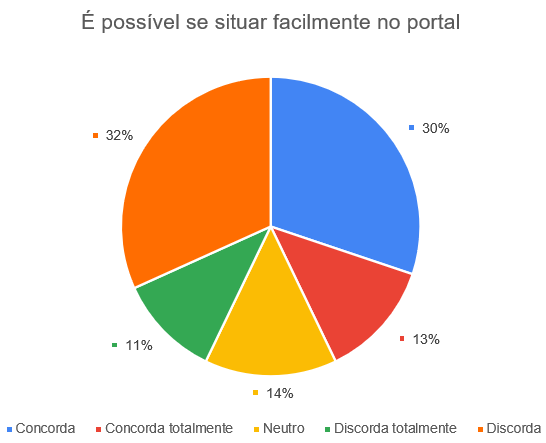
\includegraphics[width=\textwidth,frame]{img10.png}
		\caption{Se situando no Portal}
		\label{fig:grafico7}
	\end{minipage}
	\begin{minipage}{.4\columnwidth}
		\centering
		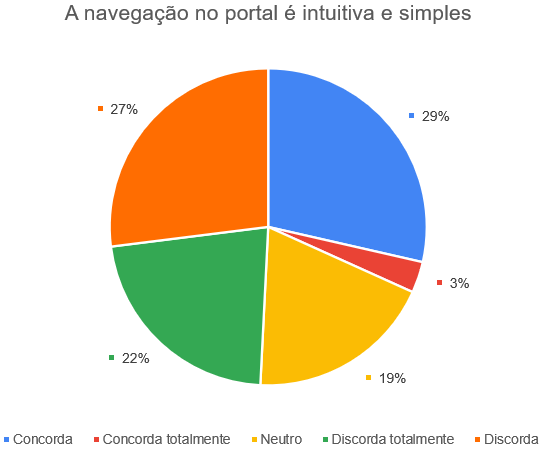
\includegraphics[width=\textwidth,frame]{img11.png}
		\caption{Facilidade de navegação no Portal}
		\label{fig:grafico8}
	\end{minipage}
\end{figure}
Com isso, evidenciamos que o critério Facilidade de recordação não está otimizado como deveria, tendo em vista que o Portal é uma ferramenta fundamental para os alunos. Como pode ser visto na Figura 10, houve um empate entre os entrevistados que acham que é facilmente possível se situar no Portal e os que não acham.

Partindo para o último ponto de análise deste capítulo, vamos apresentar o resultado das respostas sobre o questionamento da facilidade de navegação no Portal. Observe a Figura 11.

Um fator muito importante dentro dos critérios de Usabilidade é o de Segurança no uso. Para \citeonline{nielsen}, os sistemas devem ser seguros para utilizar e não devem induzir o usuário ao erro.  

Como mostrado na Figura 11, 49\% dos entrevistados discordam que a navegação no Portal seja simples e intuitiva. Um site que não possui essas características pode induzir o usuário a cometer algum tipo de erro, tornando, assim, o site inseguro para a utilização do usuário.

Optamos por segmentar este capítulo para tratar os itens avaliados positivamente pelos usuários. Portanto, a análise continuará no tópico seguinte para evidenciar a opinião dos alunos.

\subsection{Análises Positivas dos Usuários}
Ao verificarmos os resultados positivos de nossa pesquisa, foi possível identificar o critério de Facilidade de aprendizagem como o mais bem avaliado pelos alunos e confirmado por nós a partir do referencial teórico utilizado. 

De acordo com \citeonline{nielsen}, esse critério pode ser definido como a facilidade de aprender e iniciar a utilizar um sistema. Acompanhe os resultados obtidos:

\begin{figure}[!htb]
\centering
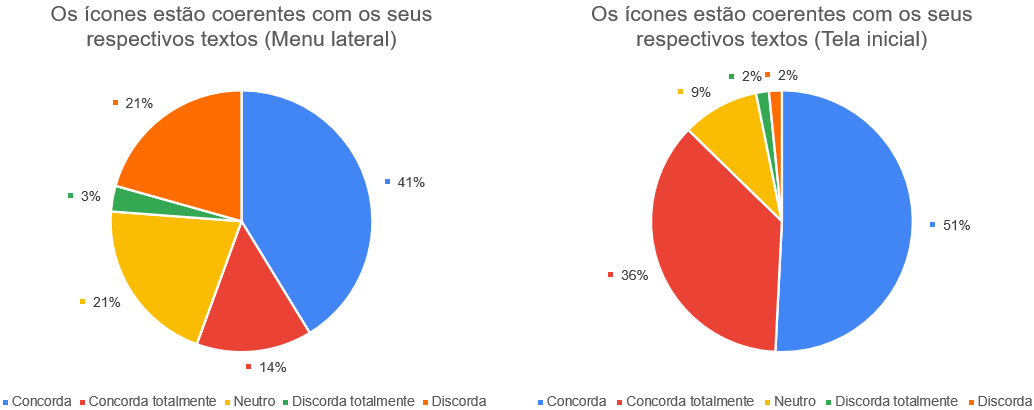
\includegraphics[scale=0.4,frame]{img12.png}
\caption{Coerência dos ícones}
\label{fig:grafico9}
\end{figure}
\begin{figure}[!htb]
\centering
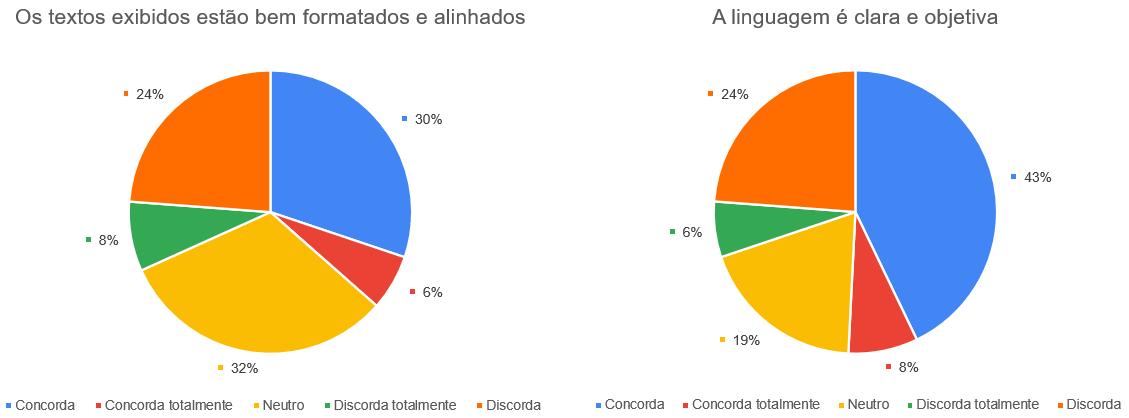
\includegraphics[scale=0.4,frame]{img13.png}
\caption{Textos do Portal}
\label{fig:grafico10}
\end{figure}
Conforme podemos ver na Figura 12, a 62\% dos entrevistados consideram que os ícones do Menu Lateral são coerentes com seus respectivos textos e 87\% dos entrevistados têm a mesma opinião sobre os ícones da Tela Inicial. Isso pode significar que mesmo na ausência dos textos os ícones ativariam na mente dos usuários a função que eles representam. 

Essa coerência dos ícones associada à disposição dos textos e a linguagem clara e objetiva que foram avaliadas positivamente pelos usuários, influenciam na função de facilidade de aprendizagem na utilização do sistema. Destacamos, então, o critério Facilidade de aprendizagem com uma potencialidade do Portal UCSal.

No capítulo a seguir, discorreremos sobre as análises feitas até aqui evidenciando algumas melhorias que podem ser aplicadas ao Portal a fim de torná-lo eficiente para o uso.


\section{Melhorias para o Portal: Sugestões e Protótipo\label{sec:sugestoesportal}}
Após a análise descrita acima, identificamos possíveis pontos de melhorias para o Portal.
Com base nesses pontos e no referencial teórico, apresentaremos, abaixo, algumas sugestões e um protótipo para um portal mais responsivo e focado na usabilidade do usuário. 

\subsection{Sugestões}
As nossas sugestões impactam profundamente em um dos critérios mais importantes de Usabilidade, a Eficiência.

A Eficiência “diz respeito ao tempo necessário para conclusão de uma atividade com apoio computacional.” \cite[p. ~53]{barbosa}. Dessa forma, para tornarmos o Portal mais eficiente para uso, acreditamos que o primeiro ponto a ser melhorado é a implementação de um design responsivo no Portal do Aluno, visto que, de acordo com a nossa pesquisa, 48\% dos acessos realizados ao sistema se originam de um Smartphone ou Tablet. 

Por isso, é fundamental que o sistema esteja preparado para receber esses acessos e consiga dispor corretamente todo o conteúdo para o usuário, independente do tamanho da tela que ele esteja acessando o sistema.

Outro ponto importante, seria a modernização do design do Portal. Tal modernização ajudaria a resolver outros dois problemas identificados: de navegação não intuitiva e de poder se localizar facilmente no Portal. 

A modernização se faz necessária pois a tecnologia está evoluindo rapidamente e os sistemas precisam se adaptar às mudanças e às tendências do mercado. As tecnologias estão focando no usuário e não no sistema. O design centrado no usuário seria um bom processo a ser adotado na hora de se propor essa modernização, pois:
\begin{quoting}[rightmargin=0cm,leftmargin=4cm]
{\footnotesize 
O Design Centrado no Usuário (User Centered Design — UCD) é um processo de design que se concentra nas necessidades e requisitos dos usuários. O uso constante de fatores humanos, ergonomia, engenharia de usabilidade e outras técnicas são o que mantém o UCD girando em torno dos usuários. 
O objetivo é produzir sistemas altamente utilizáveis e acessíveis, visando a satisfação do usuário, evitando quaisquer possíveis efeitos negativos sobre a saúde, a segurança e o desempenho. \cite{guimaraes}}
\end{quoting}
Focar no usuário em um site como o Portal do Aluno, que é a principal fonte de consulta de dados acadêmicos e financeiros é importantíssimo para oferecer aos alunos uma ótima experiência de usuário. 

\subsection{Protótipo}
A partir das sugestões mencionadas acima, desenvolvemos um protótipo que visa materializar as sugestões já mencionadas.  Embora a nossa proposta de design modernizado não apresente todas as telas do Portal devido a uma limitação do formato deste trabalho, as telas descritas abaixo podem ser um ponto de partida para um Portal com layout responsivo, focado na Usabilidade e na Experiência do Usuário.

\begin{figure}[!htb]
  \centering
  \subfloat[Atual.]{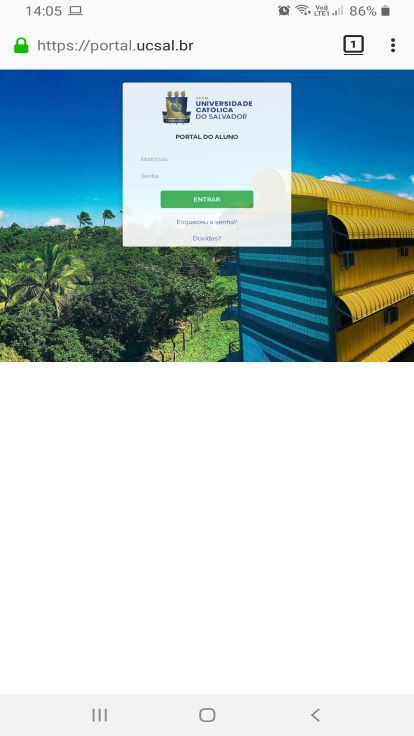
\includegraphics[scale=0.335,frame]{ALogin.jpg}\label{fig:loginantigo}}
  \qquad
  \subfloat[Protótipo.]{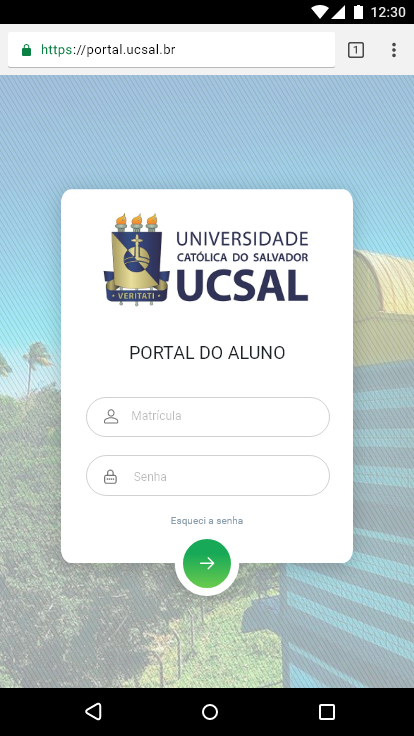
\includegraphics[scale=0.25,frame]{Login.png}\label{fig:loginprototipo}}
  \caption{Comparativo entre as telas de Login.}
  \label{figura14}
\end{figure}

Como podemos ver na Figura\ref{figura14} um comparativo entre a tela de login Atual\textbf{(a)}, sem responsividade e a tela de login do Protótipo\textbf{(b)}, atualizada e responsiva, otimizada para se adaptar ao formato de qualquer tamanho de tela e com um layout mais moderno.

\begin{figure}[!htb]
  \centering
  \subfloat[Atual.]{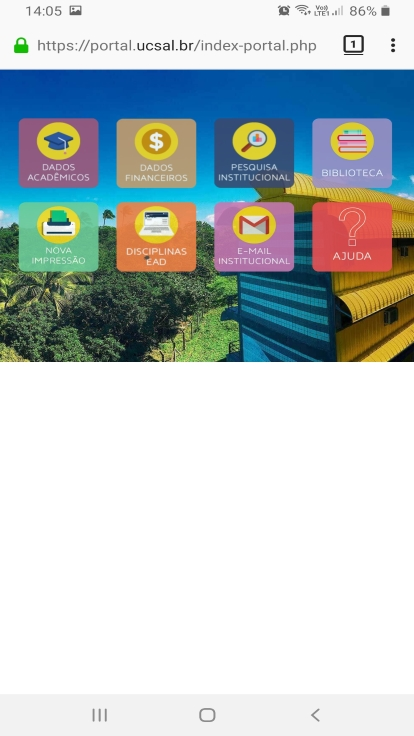
\includegraphics[scale=0.335,frame]{AInicial.jpg}\label{fig:inicialantiga}}
  \qquad
  \subfloat[Protótipo.]{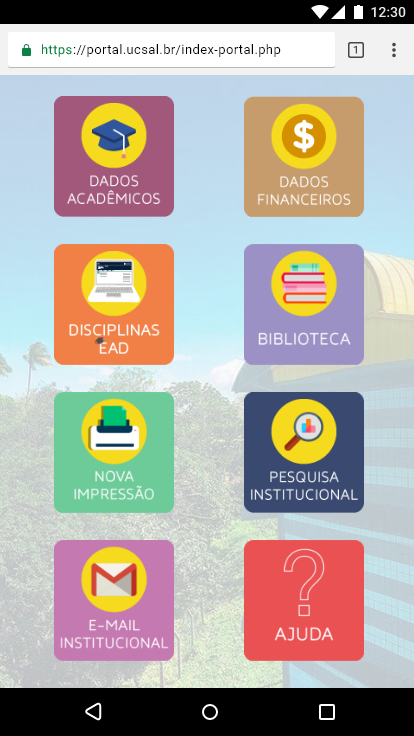
\includegraphics[scale=0.25,frame]{Inicial.png}\label{fig:inicialprototipo}}
  \caption{Comparativo entre as telas iniciais.}
  \label{figura15}
\end{figure}
Na Figura \ref{figura15}, podemos observar a diferença na exibição dos links na tela inicial do Portal, no Protótipo\textbf{(b)}, os ícones estão dispostos de maneira a ocupar toda a extensão da tela, deixando assim a visibilidade melhor para o usuário.

\begin{figure}[!htb]
  \centering
  \subfloat[Atual.]{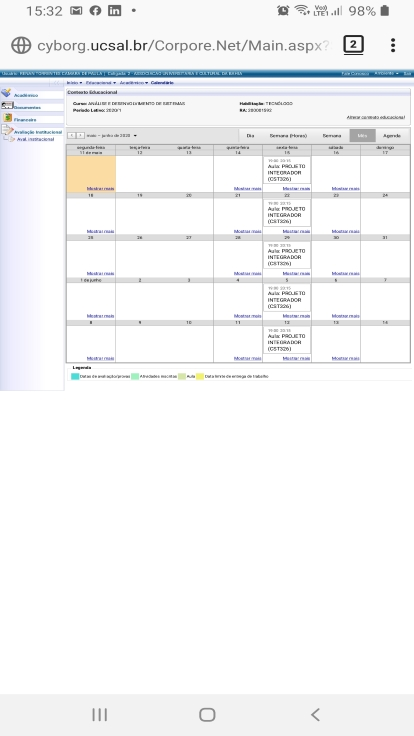
\includegraphics[scale=0.335,frame]{AMenu.jpg}\label{fig:menuantigo}}
  \qquad
  \subfloat[Protótipo.]{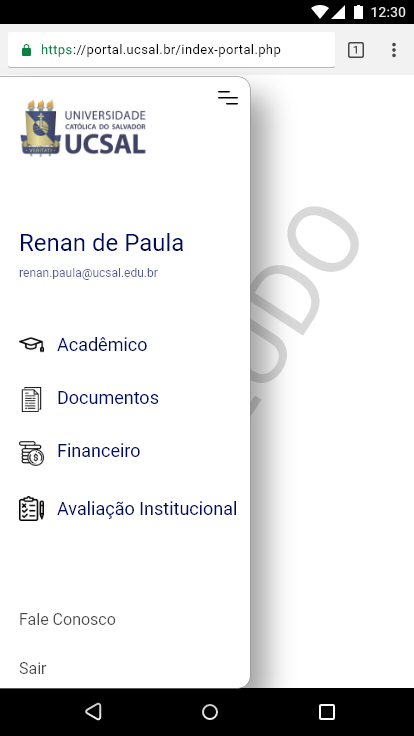
\includegraphics[scale=0.25,frame]{Menu1.png}\label{fig:menuprototipo}}
  \caption{Comparativo entre os menus do Portal.}
  \label{figura16}
\end{figure}
Podemos observar na Figura \ref{figura16} que o menu principal Atual\textbf{(a)} do Portal não se adapta ao tamanho da tela do celular, ficando com um tamanho de exibição muito pequeno e forçando o usuário a redimensionar a tela manualmente para poder clicar nos menus sem correr o risco de dar um clique errado. Na tela do Protótipo\textbf{(b)}, o novo menu é apresentado como uma aba flutuante,  um layout moderno e responsivo que se adapta automaticamente ao tamanho da tela do usuário.

\begin{figure}[!htb]
  \centering
  \subfloat[Atual.]{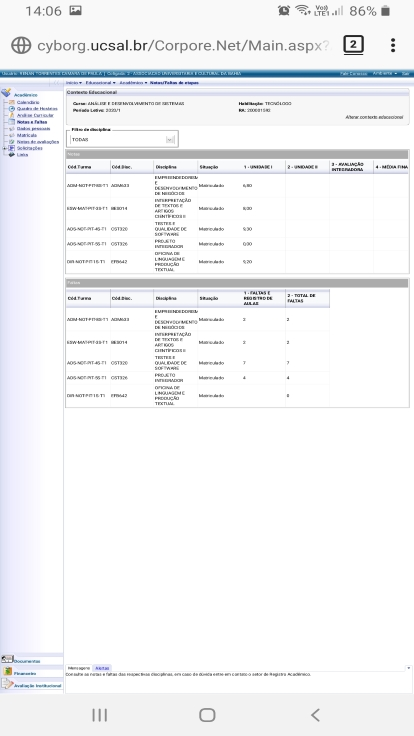
\includegraphics[scale=0.335,frame]{ANotas.jpg}\label{fig:notasantigo}}
  \qquad
  \subfloat[Protótipo Expandido.]{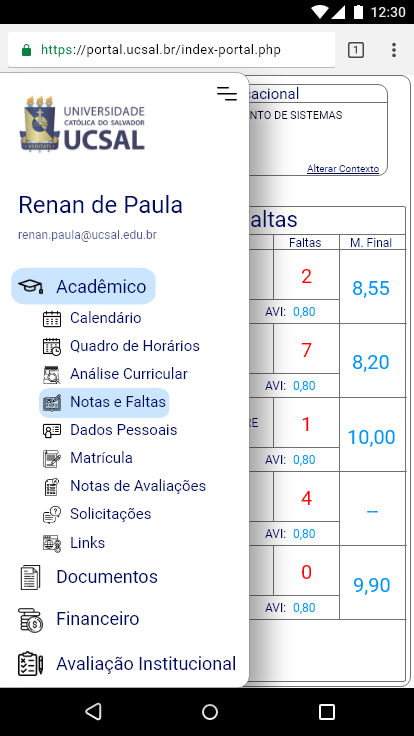
\includegraphics[scale=0.25,frame]{Notas1.png}\label{fig:notas1prototipo}}
   \qquad
  \subfloat[Protótipo Recolhido.]{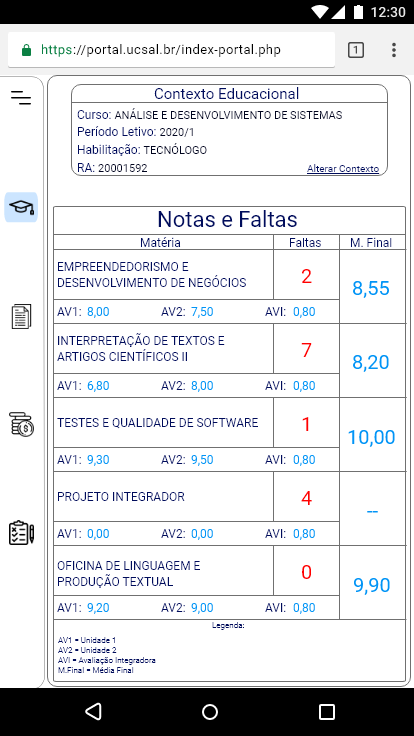
\includegraphics[scale=0.25,frame]{Notas2.png}\label{fig:notas2prototipo}}
  \caption{Comparativo entre a tela de Notas do Portal.}
  \label{figura17}
\end{figure}
Como último exemplo, temos a Figura \ref{figura17}, demostrando a exibição de uma funcionalidade no Portal Atual\textbf{(a)}; no Protótipo\textbf{(b)} com o menu expandido e no \textbf{(c)} com o menu recolhido. 

Observe que no modo de navegação atual, as informações são exibidas sem o correto redimensionamento da tela, caso o usuário deseje verificar as informações, ele precisa realizar essa função manualmente. Já no Protótipo, temos os exemplos do menu expandido, mostrando todas as funcionalidades dispostas corretamente no menu flutuante e do menu recolhido, mantendo a rastreabilidade da onde o usuário se encontra. As informações dispostas também estão otimizadas para serem exibidas corretamente na tela do usuário.

\section{Considerações Finais\label{sec:consideracoes}}
O objetivo desse trabalho foi analisar o Portal do Aluno da UCSal a partir da percepção dos alunos e também do conceito e dos critérios de Usabilidade. Constatamos que dos 5 critérios analisados 4 precisam ser melhorados e apenas 1 foi avaliado positivamente. 

Para que este trabalho resulte em uma contribuição significativa para Universidade Católica do Salvador fizemos algumas sugestões que podem ser aprofundadas e futuramente aplicadas, perante à análises, ao Portal do Aluno. Para demostrar a aplicação dessas sugestões, desenvolvemos um protótipo com foco na experiência do usuário e que pode ser utilizado como referência para a modernização do Portal, tendo em vista que ele foi projeto a partir dos resultados das pesquisas feitas com os alunos.

Destacamos que o objeto de estudo pode ser analisado a partir de outros conceitos da IHC, como Acessibilidade e Comunicabilidade. Além dessas, estudos na área da Arquitetura da Informação, Webdesign, UX, DCU e outras teorias da Tecnologia da Informação. 

A pesquisa aqui desenvolvida pode servir como um suporte para outros trabalhos que serão realizados sobre o mesmo objeto de estudo. 

\bibliographystyle{sbc}
\bibliography{sbc-template}

\end{document}
